% -*- fill-column: 52 -*-
% (local-set-key (kbd "C-c C-f") 'display-fill-column-indicator-mode)
\chapter{Haladó eszközök}
Ebben a leckében meg fogunk vizsgálni néhány olyan technikát,
amelyekkel a programok hatékonyabbá vagy egyszerűbbé tehetőek,
illetve szó lesz néhány fontos beépített szabályról is.

\section{Különbség-listák}
Listákat lehet két lista különbségeként ábrázolni,
így pl.~leírható az \pr{[1,2,3]} lista úgy, mint az
\pr{[1,2,3,8]} és \pr{[8]} listák különbsége, vagy
az \pr{[1,2,3]} és \pr{[]} listáké, vagy általánosan
az \pr{[1,2,3|M]} és \pr{M} különbségeként. A két
tagot összekapcsolhatjuk pl.~a \pr{-} operátorral:
\pr{[1,2,3|M]-M}.

Ennek az ábrázolásnak nagy előnye, hogy közvetlenül
tudunk hivatkozni a lista végére, ezért bizonyos
műveleteket sokkal hatékonyabban meg lehet
valósítani a segítségükkel, mint ha csak sima
listákat használnánk.

Egy egyszerű példa erre a hozzáfűzés:
\begin{program}
hozzáfűz_kl(X-Y, Y-Z, X-Z).
\end{program}
Ehhez persze az kell, hogy a szabály argumentumként
különbség-listákat kapjon:
\begin{query}
?- hozzáfűz_kl([a,b,c|M]-M, [1,2]-[], L-[]).
M = [1, 2],
L = [a, b, c, 1, 2]
\end{query}

Mi is történik itt pontosan? Legjobban talán akkor
látszik, ha a 3.~leckében a listák bevezetésénél
használt prefix jelöléssel írjuk fel:
\begin{query}
?- hozzáfűz_kl(lista(a, lista(b, lista(c, M)))-M,
               lista(1, lista(2, vége))-vége,
               L-vége).
\end{query}
A szabály alapján az \pr{M} és \pr{lista(1, lista(2,
  vége))} egyesül, tehát a \pr{hozzáfűz\_kl}
szabályban szereplő \pr{X} értéke
\begin{query}
lista(a,lista(b,lista(c,lista(1,lista(2,vége)))))
\end{query}
lesz, ami éppen a két lista összefűzése. Ugyanez
többszörös összefűzésre is használható, pl.
\begin{query}
?- hozzáfűz_kl([a,b|M1]-M1, [c,d|M2]-M2, L-M),
   hozzáfűz_kl(L-M, [e,f|M3]-M3, X-[]).
L = X, X = [a, b, c, d, e, f],
M = M2, M2 = [e, f],
M1 = [c, d, e, f],
M3 = []
\end{query}

A hozzáfűzésnek ezt a módját -- mivel annyira
egyszerű -- nem szokás így külön szabályként
felírni, hanem általában a programba közvetlenül
építik be, ahogy azt mindjárt látni fogjuk a
gyorsrendezésnél.

\subsection*{Gyorsrendezés}
Az előző leckében látott gyorsrendezés is sokkal
hatékonyabbá tehető ezzel a technikával. Eredetileg
így nézett ki:
\begin{program}
rendez2([], []).
rendez2([X|M], Y) :-
    szétoszt(X, M, Kicsi, Nagy),
    rendez2(Kicsi, K),
    rendez2(Nagy, N),
    hozzáfűz(K, [X|N], Y).
\end{program}
Írjuk át különbség-listák használatával!
\begin{program}
rendez2(X, Y) :- rendez2_kl(X, Y-[]).

rendez2_kl([], X-X).
rendez2_kl([X|M], Y-Z) :-
    szétoszt(X, M, Kicsi, Nagy),
    rendez2_kl(Kicsi, Y-[X|Y1]),
    rendez2_kl(Nagy, Y1-Z).
\end{program}
Látszik, hogy itt már nincsen szükség hozzáfűzésre,
a két rekurzív hívás eleve ,,jó helyre'' készíti a
megoldásait. Ezért a varázslatért a változók
egyesítése a felelős.

\subsection*{Lista megfordítása}
A \pr{fordított} szabállyal már találkoztunk a
3.~lecke egyik feladatában. Egy lehetséges megoldás
a következő:
\begin{program}
fordított1([], []).
fordított1([X|M], Y) :-
    fordított1(M, M1), hozzáfűz(M1, [X], Y).
\end{program}
Ez így nem túl hatékony. Ezt is megpróbálhatjuk
vég-rekurziós formára hozni egy plusz
(ún.~\emph{akkumulátor}) argumentum segítségével:
\index{akkumulátor}\index{\pr{fordított}}
\begin{program}
fordított2(X, Y) :- fordított2(X, [], Y).

fordított2([], Y, Y).
fordított2([X|M], F, Y) :- fordított2(M, [X|F], Y). 
\end{program}

Egy másik lehetőség, hogy különbség-listákat
használunk:
\begin{program}
fordított3(X, Y) :- fordított_kl(X, Y-[]).

fordított_kl([], X-X).
fordított_kl([X|M], Y-Z) :- fordított_kl(M, Y-[X|Z]).
\end{program}

Ha most összehasonlítjuk a két megoldást, látszik,
hogy a kettő lényegében megegyezik, csak a
vég-rekurziós változat harmadik és második
paraméterét összevontuk egy különbség-listává.

\begin{problem}
Írd át a 3.~lecke feladatai közt szereplő
\pr{lapít} szabályt hatékonyabbra különbség-listák
használatával!
\end{problem}
\begin{problem}
Oldd meg Dijkstra \emph{holland zászló}
problémáját: piros, fehér és kék színű elemek
listáját rendezzétek át úgy, hogy a piros elemek
után jöjjenek a fehérek, és végül a kékek, de ezen
belül a sorrendjük ne változzon! Például:
\begin{query}
?- holland([piros(alma),fehér(fal),kék(tenger),
            piros(paprika),fehér(holló)], X).
X = [piros(alma), piros(paprika), fehér(fal),
     fehér(holló), kék(tenger)]
\end{query}
A megoldáshoz használj különbség-listákat!
\end{problem}

\begin{infobox}{}{Dijkstra}
Edsger W.~Dijkstra (1930-2002) nevét legtöbben a
\emph{Dijkstra-algoritmus} kapcsán ismerik. Ez egy
úthálózatban (súlyozott gráfban) megkeresi két pont
között a legrövidebb utat.\index{Dijkstra}
\end{infobox}

\section{Kifejezések vizsgálata}
Egy kifejezés típusának megvizsgálására a következő
beépített szabályok adottak:
\begin{itemize}
\item \pr{var(X)} : \pr{X} változó (és nincs értéke)
\item \pr{nonvar(X)} : \pr{X} nem változó vagy van értéke
\item \pr{atom(X)} : \pr{X} atom
\item \pr{number(X)} : \pr{X} szám
  \begin{itemize}
    \item \pr{integer(X)} : \pr{X} egész szám
    \item \pr{float(X)} : \pr{X} valós szám
  \end{itemize}
\item \pr{atomic(X)} : \pr{X} atom vagy szám
\item \pr{compound(X)} : \pr{X} összetett struktúra
\end{itemize}
\index{\pr{var}}\index{\pr{nonvar}}
\index{\pr{atom}}\index{\pr{number}}
\index{\pr{integer}}\index{\pr{float}}
\index{\pr{atomic}}\index{\pr{compound}}
Egy struktúra ezen kívül szétszedhető az elemeinek
listájára (fej + argumentumok), illetve
visszaépíthető ezekből az \pr{=..} segítségével:
\index{\pr{=..}}
\begin{query}
?- f(a,b,c) =.. X.
X = [f, a, b, c]
?- X =.. [f, a, b, c].
X = f(a,b,c)
\end{query}

A funktort és aritást, illetve az egyes
argumentumokat külön is le lehet kérdezni a
\pr{functor} ill. \pr{arg} használatával:
\index{\pr{functor}}\index{\pr{arg}}
\begin{query}
?- functor(f(a,b,c), F, N).
F = f,
N = 3
?- arg(1, f(a,b,c), X).
X = a
?- arg(2, f(a,b,c), X).
X = b
\end{query}
Ezeknek a segítségével a struktúrákat tudjuk fix
hosszú \emph{tömbökként} kezelni, tehát olyan
adattárolókként, amelyeknek tetszőleges eleme
hatékonyan elérhető (ellentétben a listákkal, ahol
egy elem eléréséhez előbb végig kell mennünk
az összes előtte levőn).\index{tomb@tömb}
Például a
\begin{query}
?- functor(T, t, 10), arg(5, T, 42)
\end{query}
hatására a \pr{T} egy olyan 10-elemű tömb lesz,
amelynek az 5.~eleme a 42.

\subsection*{Csere}
Hogyan lehetne ezek segítségével megoldani a
következő feladatot: egy kifejezésben egy másik
(al)kifejezés minden előfordulását le akarjuk
cserélni valami másra. Például:
\begin{query}
?- lecserél(sin(x), t, 2*sin(x)*f(sin(x)), F).
F = 2*t*f(t)
\end{query}
Itt az ,,előfordulás'' egyesíthetőséget jelent,
tehát
\begin{query}
?- lecserél(a+b, v, f(a,A+B), F).
A = a,
B = b,
F = f(a, v)
\end{query}

Három eset van:
\begin{enumerate}
\item A kifejezés és a lecserélendő alkifejezés
  megegyezik -- az egészet cseréljük.
\item A kifejezés atom/szám -- nincs mit csinálni.
\item A kifejezés egy struktúra; az argumentumaira
  kell elvégezni a cserét.
\end{enumerate}
Ez alapján a három szabály:
\begin{program}
lecserél(X, Y, X, Y) :- !.
lecserél(_, _, Z, Z) :- atomic(Z), !.
lecserél(X, Y, Z, Z1) :-
    Z =.. [F|Arg],
    mindent_lecserél(X, Y, Arg, Arg1),
    Z1 =.. [F|Arg1].
\end{program}
A \pr{mindent\_lecserél} szabály egy lista minden
elemére elvégzi a cserét:
\begin{program}
mindent_lecserél(_, _, [], []).
mindent_lecserél(X, Y, [Z|M], [Z1|M1]) :-
    lecserél(X, Y, Z, Z1),
    mindent_lecserél(X, Y, M, M1).
\end{program}
Ennek segítségével készíthetünk függvénykiértékelőt:
\begin{query}
?- kiértékel(x*sin((x+y)/2), [x=1,y=2.14], X).
X = 0.9999996829318346
\end{query}
A második argumentumban \pr{szimbólum = szám}
alakban vannak megadva a helyettesítési értékek.
\begin{program}
kiértékel(K, L, X) :-
    behelyettesít(K, L, K1), X is K1.

behelyettesít(K, [], K).
behelyettesít(K, [A=N|M], K2) :-
    lecserél(A, N, K, K1),
    behelyettesít(K1, M, K2).
\end{program}

\begin{problem}
Írj szabályt, ami egy összeadásokat
tartalmazó kifejezést egyszerűsít úgy, hogy az
ismeretleneket (ha lehet) összevonja és előre
rakja, a többi összeadást pedig elvégzi!
(Vigyázat, ez egy elég komplex feladat!)
\begin{query}
?- egyszerűsít(1+1+a, E).
E = a+2
?- egyszerűsít(1+a+4+2+b+c, E).
E = a+b+c+7
?- egyszerűsít(3+x+x, E).
E = 2*x+3
\end{query}
\end{problem}

\section{Magasabb rendű szabályok}
Vannak olyan szabályok, amelyek argumentumként egy
másik szabályt (célt, kérdést) várnak. Ilyen volt
például a tagadás, de van még néhány másik is.

\subsection*{Listakezelés}
Egy nagyon hasznos szabály a \pr{maplist}, ami egy
lista összes elemére megnézi, hogy teljesít-e egy
adott szabályt, pl.
\index{\pr{maplist}}
\begin{query}
?- maplist(number, [3,4,5]).
true
?- maplist(number, [3,a,5]).
false
\end{query}
A szabály lehet többargumentumú is, ilyenkor több
listát kell megadni, egyet minden argumentumhoz. A
\pr{mindent\_lecserél} például megfogalmazható így:
\begin{program}
mindent_lecserél(X, Y, Z, Z1) :-
    maplist(lecserél(X, Y), Z, Z1).
\end{program}
Itt a \pr{lecserél} első két argumentumát előre
megadtuk, a maradék kettőt a \pr{Z} és \pr{Z1}
listákból veszi ki.

\subsection*{Összes megoldás}
Gyakran előfordul, hogy az összes megoldásra
kíváncsiak vagyunk. Ilyenkor ezeket egy listában le
lehet kérni a \pr{bagof} (,,zsákja''), \pr{setof}
(,,halmaza'') vagy \pr{findall} (,,találd meg az
összeset'') segítségével. Nézzük meg sorban őket!

A \pr{bagof(X, P, L)} megkeresi az összes olyan
\pr{X}-et, amire \pr{P} igaz, és \pr{L} ezeknek a
listája. Például:
\index{\pr{bagof}}
\begin{program}
életkor(lica, 11).
életkor(mimi, 10).
életkor(dusa, 5).
életkor(zsófi, 5).
életkor(juli, 2).
\end{program}
\begin{query}
?- bagof(X, életkor(X, 5), L).
L = [dusa, zsófi]
?- bagof(X, életkor(X, _), L).
L = [juli]
\end{query}
További megoldásokként megkapjuk életkorok szerint
csoportosítva a többi gyereket is. Ha azt
szeretnénk, hogy egyszerre az összes gyereket
megkapjuk, akinek ismert az életkora (és nem csak
azokat, akiknek azonos), akkor erre egy speciális
jelölést kell használni:
\begin{query}
?- bagof(X, N^életkor(X, N), L).
L = [lica, mimi, dusa, zsófi, juli]
\end{query}
Az \pr{N\textasciicircum} itt azt jelenti, hogy
,,van olyan \pr{N}, amire igaz, hogy \dots''.

A \pr{setof} nagyon hasonló ehhez, de az azonos
elemekből csak egyet tart meg, például:
\index{\pr{setof}}
\begin{query}
?- bagof(N, X^életkor(X, N), L).
L = [11, 10, 5, 5, 2]
?- setof(N, X^életkor(X, N), L).
L = [2, 5, 10, 11]
\end{query}

Végül a \pr{findall} olyan, mint a \pr{bagof},
amikor a kifejezés egy változójának értéke sincs
lekötve, tehát mintha minden (nem keresett) \pr{V}
változóhoz oda lenne írva a
\pr{V\textasciicircum}. Például:
\index{\pr{findall}}
\begin{query}
?- bagof(X, N^életkor(X, N), L).
L = [lica, mimi, dusa, zsófi, juli]
?- findall(X, életkor(X, _), L).
L = [lica, mimi, dusa, zsófi, juli]
\end{query}

\begin{problem}
Írj szabályt, ami a \pr{bagof} segítségével
megkeresi egy halmaz (lista) összes részhalmazát!
\end{problem}

\section{Dinamikus szabályok}
Szabályokat a program futása közben automatikusan is
hozzá lehet adni az adatbázishoz, illetve ki lehet
venni belőle. Ha a szabály már létezik, akkor ehhez
az kell, hogy \emph{dinamikusnak} legyen beállítva,
pl.:
\index{\pr{dynamic}}
\begin{program}
:- dynamic foo/2. % 2 aritású
\end{program}
Ezután az alábbi módon lehet a \pr{foo} szabályait
módosítani:
\begin{itemize}
\item \pr{asserta(foo([], \_))} : az adatbázis
  elejére teszi a \pr{foo([], \_).} tényt.
\item \pr{assertz(foo(X, Y) :- X > Y)} : az
  adatbázis végére teszi a \pr{foo(X, Y) :- X > Y.}
  szabályt.
\item \pr{retract(foo([], \_))} : törli a
  \pr{foo([], \_).} tényt.
\item \pr{retractall(foo(\_,\_))} : törli az összes
  szabályt, aminek a feje egyesíthető a
  \pr{foo(\_,\_)}-val.
\end{itemize}
\index{\pr{asserta}}\index{\pr{assertz}}
\index{\pr{retract}}\index{\pr{retractall}}
Ezek segítségével például definiálhatjuk magunk is a
\pr{findall} szabályt:
\begin{program}
összes(X, Cél, L) :-
    Cél, assertz(tároló(X)), fail
  ; assertz(tároló(nincs_több)), összegyűjt(L).

összegyűjt(L) :-
    retract(tároló(X)), !,
    ( X = nincs_több, !, L = []
    ; L = [X|M], összegyűjt(M)
    ).
\end{program}
\begin{query}
?- összes(X, életkor(X, _), L).
L = [lica, mimi, dusa, zsófi, juli]
\end{query}

Ez a megoldás feltételezi, hogy a \pr{tároló}
szabály még nem létezett, és hogy a keresett értékek
közt nem szerepelhet a \pr{nincs\_több} atom. Ezt
elkerülendő, ezeket a \pr{\$} prefix operátorral
szokás megkülönböztetni, tehát \pr{tároló(X)}
helyett \pr{\$tároló(X)} és \pr{nincs\_több} helyett
\pr{\$nincs\_több} (vagy a zárójelet kiírva
\pr{\$(tároló(X))} és \pr{\$(nincs\_több)}).

Az önmagát módosító programok megértése nehéz, ezért
az ilyen jellegű technikákat csak jól elkülönített
programrészekben ajánlott alkalmazni.

\subsection*{Polipos játék}

\begin{wrapfigure}[7]{r}{.35\textwidth}
  \centering
  \vspace{-4em}
  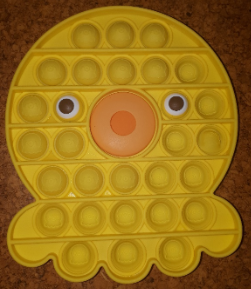
\includegraphics[width=.33\textwidth]{images/polip.png}
\end{wrapfigure}
A játéktáblán sorokba rendezve kidudorodó gombok találhatóak.
A játékosok felváltva lépnek, és egy lépés során kiválasztanak egy sort,
és abban a sorban tetszőleges számú (de legalább egy) gombot benyomnak.
Az veszt, aki az utolsó gombot nyomja be.

Írjunk programot, ami megtalálja a legjobb lépést! Ehhez először írjuk le a táblát:
\begin{program}
polip([3,5,2,4,5,5,3]).
\end{program}
A lista minden eleme az adott sorban levő gombok számának felel meg.
Adjunk hozzá logikát is:
\begin{program}
nyertes([]) :- !. 
nyertes(L) :- nyom(L, _, L1), vesztes(L1), !.
\end{program}
Akkor nyer az aktuális játékos, ha (i)~már nincsen benyomható gomb, vagy
(ii)~ha tud vesztes állást előidézni.

A \pr{nyom(L, I-N, L1)} reláció akkor teljesül, ha az \pr{L} állásban
az \pr{I}-edik sorban \pr{N} gombot benyomva az \pr{L1} állás jön létre.
A sorok számlálásához felveszünk egy második paramétert, ami 1-ről indul:
\begin{program}
nyom(L, V, L1) :- nyom(L, 1, V, L1).
\end{program}
A lépéskor három lehetőség van:
\begin{enumerate}
\item Benyomjuk az egész első sort.
\item Benyomunk valamennyit az első sorból (de nem mindet).
\item Másik sorban nyomunk.
\end{enumerate}
Ennek megfelel az alábbi három szabály:
\begin{program}
nyom([X|M], I, I-X, M).
nyom([X|M], I, I-Y, [Y1|M]) :-
    X1 is X - 1, között(1, X1, Y), Y1 is X1 - Y.
nyom([X|M], I, V, [X|M1]) :-
    I1 is I + 1, nyom(M, I1, V, M1).
\end{program}

A vesztes állás az egyszerűen a nem nyertes állás:
\begin{program}
vesztes(L) :- \+ nyertes(L).
\end{program}

Végül pedig nyerő lépés az, ami után vesztes állás jön létre:
\begin{program}
nyerő_lépés(L, V) :- nyom(L, V, X), vesztes(X), !.
\end{program}

Például a kezdőállásból egy nyerő lépést így kaphatunk meg:
\begin{query}
?- polip(P), nyerő_lépés(P, X).
P = [3, 5, 2, 4, 5, 5, 3],
X = 1-3. % Az első sorban nyomjuk be az összeset (3)
\end{query}

De mi köze mindennek a dinamikus szabályokhoz?
Ha valaki kipróbálja a fenti programot, bizony elég sokat kell várnia,
mert nagyon lassú. Fel lehetne gyorsítani azzal, ha a \pr{vesztes}
már kiszámolt értékeit (tehát, hogy mely állások vesztesek) eltárolnánk,
és amikor újra szükség van rájuk, akkor egyszerűen csak elő tudnánk húzni
az eredményt a tarsolyunkból. Ezt a módszert -- a korábban kiszámolt
eredmények eltárolását -- \emph{memoizálás}\/nak vagy \emph{táblázás}\/nak
szokás nevezni.\index{memoizálás}\index{tablazas@táblázás}

A legtöbb Prolog rendszernek van erre valamilyen beépített módszere,
pl.~\name{SWI-Prolog}ban mindössze annyit kell írni, hogy
\begin{program}
:- table vesztes/1.
\end{program}
$\dots$ de ez nem szabványos. A dinamikus szabályok segítségével viszont
ez nagyon könnyen megoldható:
\begin{program}
:- dynamic(vesztes/1). 
vesztes(L) :-
    \+ nyertes(L), !,
    asserta((vesztes(L) :- !)). 
vesztes(L) :-
    asserta((vesztes(L) :- !, fail)),
    fail. 
\end{program}
Ha egy állásról kiderül, hogy vesztes, akkor ezt, mint tényt, elrakjuk.
Ha meg az derül ki, hogy nem, akkor egy olyan szabályt rakunk el,
ami ezt biztosítja; ennek az utóbbi szabálynak is \pr{fail} kell a végére,
különben a \pr{vesztes(L)} elsőre mindig igaz lenne.

Így a program már nagyon gyors. Ez természetesen egy kompromisszum:
a sebességért cserébe tárhellyel fizetünk. Ha sokkal több megjegyzendő adatunk van,
akkor a program könnyen kifuthat a memóriából.

\section{Vezérlés}
A program folyásának vezérlésére már láttunk néhány
módszert, mint a vágás (\pr{!}) vagy a mindig igaz
ill. hamis célok (\pr{true}, \pr{false} ill.~\pr{fail}).
Itt van néhány további:
\begin{enumerate}
\item Ha egy szabály több megoldást is vissza tud
  adni, de mi csak az elsőt szeretnénk, a vágással
  le tudjuk tiltani a továbbiakat. Ez elég gyakori
  ahhoz, hogy van rá egy beépített szabály, a
  \pr{once} (,,egyszer''):
  \index{\pr{once}}
\begin{program}
once(P) :- P, !.
\end{program}
\item Amikor egy \pr{P} változót célként használunk,
  mint a \pr{once} vagy a tagadás definíciójában,
  akkor valójában a háttérben a \pr{call(P)}
  (,,hív'') hívódik meg; a szabvány szerint ezt ki is kéne írni,
  de a legtöbb implementációban elhagyható. Ennek ellenére
  érdemes lehet kiírni,
  hogy egyértelműbb legyen, mi történik. Amikor a
  \pr{call}-nak több argumentuma van, ezeket a
  célhoz kapcsolandó további paraméterekként
  értelmezi, tehát pl.:
\index{\pr{call}}
\begin{query}
?- P = hozzáfűz([a,b]),
   call(P, [c,d], X),
   call(P, [x,y], Y).
P = hozzáfűz([a, b]),
X = [a, b, c, d],
Y = [a, b, x, y].
\end{query}
\item A \pr{(P -> Q; R)} jelentése: ha \pr{P}, akkor
  \pr{Q}, különben \pr{R}. Tehát pl.~az alábbi kettő
  ekvivalens:
\index{\pr{->}}
\begin{program}
implikáció(X) :- foo(X) -> bar(X); baz(X).
\end{program}   
és
\begin{program}
implikáció(X) :- foo(X), !, bar(X).
implikáció(X) :- baz(X).
\end{program}
\item A felhasználóval való kommunikációhoz gyakran
  van szükség végtelen ciklusra, ezt segíti a
  \pr{repeat} (,,ismétel''), amit így lehet
  definiálni:
\index{\pr{repeat}}
\begin{program}  
repeat.
repeat :- repeat.
\end{program}
Ez tehát mindig igaz, akárcsak a \pr{true}, de ezt
az igaz értéket végtelenszer generálja. Egy példa a
használatára az alábbi program, ami a \pr{read}
segítségével kér be a felhasználótól számokat, és
kiírja a négyzetüket, egészen amíg \pr{stop}-ot nem
kap:
\index{\pr{read}}
\begin{program}
négyzetes :-
    repeat, read(X),
    ( X = stop, !
    ; Y is X * X, write(Y), fail
    ).
\end{program}
\end{enumerate}

\section{Projekt: mankala}
Készítsünk mesterséges intelligenciát a \emph{kalah}
mankala-játékhoz!

\begin{center}
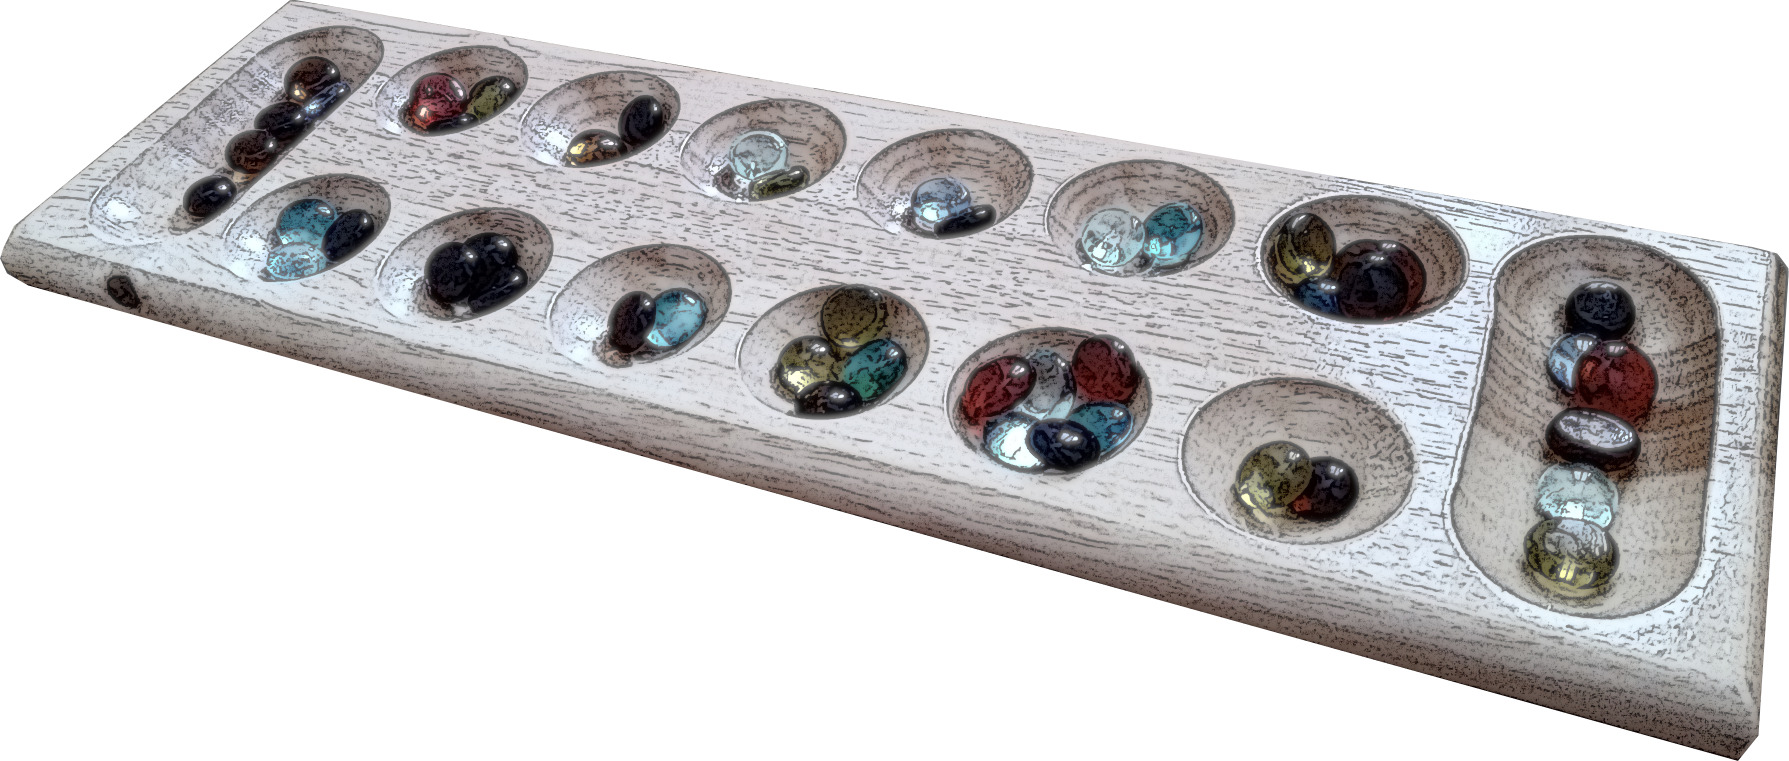
\includegraphics[width=\textwidth]{images/kalah.jpg}
\end{center}

A játéknak számos variánsa létezik, itt most egy
egyszerű változatot fogunk megvalósítani. A táblán
12 kisebb és 2 nagyobb lyuk található; az egyes
játékosokhoz a hozzájuk közelebb levő 6 lyuk és a
jobb kéz felőli nagyobb lyuk (a \emph{kalah})
tartozik. Kezdetben minden (kis) lyukban 6 kő van,
bár szokás 4--4 kővel is játszani.

A játékosok felváltva lépnek. Egy lépés abból áll,
hogy választanak egy saját lyukat, amiben van kő, és
a benne levő köveket óramutató járásával ellenkező
irányban egyesével beleszórják a következő lyukakba
-- amikor elfogynak a sajátok, akkor egy kerül a
saját kalahba, utána az ellenfél lyukaiba, és ha
azok elfogytak, akkor megint a sajátokba (az
ellenfél kalahját ki kell hagyni).

Ha az utolsó kő a (saját) kalahba esik, akkor még
egyszer lehet lépni (ez bárhányszor ismételhető). Ha
az utolsó kő egy olyan saját lyukba kerül, ami
előtte üres volt, és a szemben levő lyukban van kő,
akkor a szóró játékos mindkét lyuk tartalmát
megkapja és a kalahjába teszi.

A játékot az nyeri meg, aki megszerzi a köveknek
több, mint a felét. A játéknak akkor is vége van, ha
egy lépés végeztével az egyik térfél teljesen kiürül
-- ilyenkor a másik játékos megkapja a saját oldalán
levő köveket.

\subsection*{Keretprogram}

Ez már egy elég komplex program lesz, amit apránként
fogunk felépíteni felülről lefelé, tehát először
egy magas szinten fogalmazzuk meg, és utána
kitöltjük a részleteket.

A Kalah az absztrakt táblajátékok általános sémáját
követi; erre írhatunk egy olyan keretprogramot, ami
később akár más hasonló jellegű játékokra is
használható lesz:
\begin{program}
kalah :-
    alapbeállítás(Állás, Játékos),
    kirajzol(Állás, Játékos),
    játék(Állás, Játékos).

játék(Állás, Játékos) :-
    játék_vége(Állás, Játékos, Eredmény), !,
    bejelent(Eredmény).
játék(Állás, Játékos) :-
    lépést_választ(Állás, Játékos, Lépés),
    lép(Lépés, Állás, Állás1),
    következő_játékos(Játékos, Játékos1), !,
    kirajzol(Állás1, Játékos1),
    játék(Állás1, Játékos1).
\end{program}

Az \pr{alapbeállítás} felállítja a tábla kezdő
állapotát, és meghatározza a kezdő játékost. Ezt
az állást kirajzoljuk, és utána kezdődik a tényleges
\pr{játék/2}. Ez először ellenőrzi, hogy vége van-e
a játéknak, és ha igen, közli az
eredményt. Egyébként a soron következő játékos
választ egy lépést, ezt a lépést le is játsza, majd
a következő játékos számára kirajzolja a (módosult)
állást és a játék megy tovább.

A két játékosunk lehet az \pr{ember} és a
\pr{számítógép}, és ezek váltakoznak, tehát
\begin{program}
következő_játékos(ember, számítógép).
következő_játékos(számítógép, ember).
\end{program}

Az eredmény lehet egyszerűen a nyertes megnevezése,
vagy a \pr{döntetlen}:
\begin{program}
bejelent(ember) :- kiír('Nyertél, gratulálok!').
bejelent(számítógép) :- kiír('Nyertem.').
bejelent(döntetlen) :- kiír('Döntetlen lett!').
\end{program}

Itt a \pr{kiír} a \pr{write} olyan változata, ami
utána még egy újsort is kiír (\pr{nl}):
\begin{program}
kiír(X) :- write(X), nl.
\end{program}

\subsection*{Reprezentáció}
A legfontosabb feladat itt is, mint mindig, a
\emph{reprezentáció} (adatábrázolás) ügyes
megválasztása. Hogyan érdemes eltárolnunk az állást?
A cél, hogy később kényelmesen le tudjuk írni a
lépéseket.

Számozzuk be a lyukakat mindkét játékosnak balról
jobbra 1--6-ig. A lépés tehát mindkét játékos
számára egy 1 és 6 közötti szám lesz, vagyis
pontosabban ezeknek egy listája, ugyanis ha az
utolsó kő a kalahba kerül, akkor a játékos újra
léphet, és így egy lépést a kiválasztott lyukak
listájával lehet definiálni.

Az állást tehát a $2\times6$ lyukban, valamint a
kalahokban levő kövek számával tudjuk leírni. A
belső ábrázolásunk \pr{tábla(La, Na,Lb,Nb)} alakú
lesz, ahol \pr{La} és \pr{Lb} számok 6-elemű listája
(a lyukakban levő kövek), \pr{Na} és \pr{Nb} sima
számok (a kalahokban levő kövek). Az \pr{a}-végűek
az éppen soron következő játékoshoz tartozó adatok,
a \pr{b}-végűek az ellenfélhez tartozóak.

A játékot kezdje mindig az emberi játékos:
\begin{program}
alapbeállítás(Állás, ember) :-
    kövek_száma(K),
    Állás = tábla([K,K,K,K,K,K],0,
                  [K,K,K,K,K,K],0).

kövek_száma(6).
\end{program}

A kövek számát érdemes a fent látható módon kivenni
külön ténybe, hogy később kényelmesen változtatható
legyen.

\subsection*{A Kalah szabályai}
Mikor van vége a játéknak? Itt azt az egyszerűsítést
alkalmazhatjuk, hogy ha az egyik térfél a lépés
végére kiürül, akkor a másik térfélen levő kövek --
még a lépés részeként -- bekerülnek a megfelelő
kalahba. Elég tehát azt a feltételt megnéznünk, hogy
valamelyik játékos elvitte már a köveknek több, mint
a felét.
\begin{program}
játék_vége(tábla(_,N,_,N), _, döntetlen) :-
    kövek_száma(K), N =:= 6 * K, !.
játék_vége(tábla(_,N1,_,_), Játékos, Játékos) :-
    kövek_száma(K), N1 > 6 * K, !.
játék_vége(tábla(_,_,_,N2), Játékos, Másik) :-
    kövek_száma(K), N2 > 6 * K,
    következő_játékos(Játékos, Másik).
\end{program}

Következik a lépések leírása. Ahogy láttuk, a lépés
lyukak listájával van megadva. Ha a lista végére
értünk, akkor a másik játékos következik, ezért meg
kell ,,fordítani'' a táblát:
\begin{program}
lép([], Állás, Állás1) :- megfordít(Állás, Állás1).

megfordít(tábla(La,Na,Lb,Nb), tábla(Lb,Nb,La,Na)).
\end{program}

Egyébként pedig körbeszórjuk (,,vetjük'') a köveket:
\begin{program}
lép([L|M], Állás, Állás2) :-
    kövek(L, Állás, K),
    vet(K, L, Állás, Állás1),
    lép(M, Állás1, Állás2).
\end{program}

Itt a \pr{kövek} megadja, hogy egy adott lyukban
hány kő van:
\begin{program}
kövek(I, tábla(L,_,_,_), K) :-
    n_edik(I, L, K), K > 0.

n_edik(N, [_|M], X) :-
    N > 1, !, N1 is N - 1,
    n_edik(N1, M, X).
n_edik(1, [X|_], X).
\end{program}

A vetés a játék lelke, és egyben a legbonyolultabb
része. Ezt két részre szedjük, a saját oldalon és az
ellenfél oldalon való vetésre (utóbbi szükség
szerint újra hivatkozik majd a \pr{vet}-re):
\begin{program}
vet(Kövek, Luk, Állás, Állás2) :-
    vet_saját(Kövek, Luk, Állás, Állás1, Kövek1),
    vet_ellenfél(Kövek1, Állás1, Állás2).
\end{program}

Ez tehát azt mondja, hogy a \pr{Luk} lyukból indulva
vetünk \pr{Kövek} darab követ, és így jutunk a
kezdeti \pr{Állás}-ból a végső \pr{Állás2}-be. A
saját oldali vetés végeztekor egy közbülső
\pr{Állás1}-be jutunk, ahol még további \pr{Kövek1}
darab követ kell vetnünk az ellenfél oldalára.

Ha a kövek száma nagyobb, mint 7 $-$ \pr{Luk}, akkor
átjutunk az ellenfél oldalára (tehát az 1-es lyukból
legalább 7 kő kell, a 2-esből 6, \dots, a 6-osból
legalább 2, hiszen az első a kalahba kerül):
\begin{program}
vet_saját(Kövek, Luk, tábla(La,Na,Lb,Nb),
          tábla(La1,Na1,Lb,Nb), Kövek1) :-
    Kövek > 7 - Luk, !, % átmegy az ellenfélhez
    felvesz_és_szór(Luk, Kövek, La, La1),
    Na1 is Na + 1, Kövek1 is Kövek + Luk - 7.
\end{program}

A lényeget a \pr{felvesz\_és\_szór} végzi, amit
kicsit későbbre hagyunk. Ha nem jutunk át a másik
oldalra, akkor a megmaradó kövek száma 0:
\begin{program}
vet_saját(Kövek, Luk,
          tábla(La,Na,Lb,Nb), Állás, 0) :-
    Kövek =< 7 - Luk,
    felvesz_és_szór(Luk, Kövek, La, La1),
    elfogás(Luk, Kövek, La1, La2, Lb, Lb1, N),
    raktározás(N, Kövek, Luk, Na, Na1),
    vetés_vége(tábla(La2,Na1,Lb1,Nb), Állás).
\end{program}

Az \pr{elfogás} megnézi, hogy hány követ ejtettünk
foglyul (\pr{N}), és hogy ennek hatására hogyan
változik a tábla (új \pr{La2} és \pr{Lb1}
értékek). A \pr{raktározás} frissíti a kalah értékét
(\pr{Na1}), egyrészt az elfogott kövek, másrészt az
aktuális vetés során oda jutó kő figyelembe
vételével. Végül a \pr{vetés\_vége} ellenőrzi, hogy
kiürült-e az egyik térfél, és ha igen, akkor a
fennmaradó köveket a megfelelő kalahba teszi.

Nézzük meg ezeket sorban!
\begin{program}
elfogás(Luk, Kövek, La, La1, Lb, Lb1, N) :-
    Vége is Luk + Kövek,
    n_edik(Vége, La, 1),
    Szemben is 7 - Vége,
    n_edik(Szemben, Lb, K),
    K > 0, !, % üresbe érkeztünk és van szemben kő
    n_csere(Vége, La, 0, La1),
    n_csere(Szemben, Lb, 0, Lb1),
    N is K + 1.
elfogás(_, _, La, La, Lb, Lb, 0) :- !.

n_csere(1, [_|M], Y, [Y|M]) :- !.
n_csere(N, [X|M], Y, [X|M1]) :-
    N > 1, !, N1 is N - 1,
    n_csere(N1, M, Y, M1).
\end{program}
A \pr{Vége} adja meg, hogy melyik lyukba kerül az
utolsó kő. Ha ebben 1 kő van, tehát a vetés előtt
üres volt, akkor megvizsgáljuk, hogy szemben van-e
kő (a szemben levő lyukak számozásának iránya
fordított, ezért a megfelelő index a 7 $-$ \pr{Vége}
lesz). Ha ez is teljesül, akkor kinullázzuk ezt a
két lyukat az \pr{n\_csere(I, L, X, L1)}
használatával, ami az \pr{L} lista \pr{I}-edik
elemét \pr{X}-re állítja. Végül a kapott kövek száma
a szemben levő kövek száma + 1. Ellenkező esetben a
tábla változatlan marad és a kapott kövek száma 0
lesz.

Figyeljük meg, hogy itt az aránylag bonyolult
feltételt nem ismételjük meg a második szabályban,
hanem a procedurális olvasatra hagyatkozunk: az első
szabályban levő vágás miatt a másodikba csak akkor
jutunk, ha a feltétel nem teljesül. Ez a deklaratív
olvasatot elrontja, de megengedhető, mivel tudjuk,
hogy csak olyan környezetben használjuk, ahol az
\pr{La1}, \pr{Lb1} és \pr{N} változóknak nincsen
értéke. A hatékonyság érdekében sok szabály
használja itt ezt a módszert.

A \pr{raktározás} elég magától értetődő. Ha az
elfogott kövek száma 0, akkor ellenőrzi, hogy az
utolsó kő a kalahba került-e, egyébként csak
hozzáadja az eddigiekhez az elfogott köveket:
\begin{program}
raktározás(0, Kövek, Luk, Na, Na) :-
    Kövek < 7 - Luk, !.
raktározás(0, Kövek, Luk, Na, Na1) :-
    Kövek =:= 7 - Luk, !, Na1 is Na + 1.
raktározás(N, _, _, Na, Na1) :-
    N > 0, !, Na1 is Na + N.
\end{program}

A kiürült térfelek kezelésekor a másik térfél köveit
összeadjuk, és azt is kiürítjük:
\begin{program}
vetés_vége(tábla(La,Na,Lb,Nb),
           tábla(La,Na,La,Nb1)) :-
    üres(La), !, összeg(Lb, X), Nb1 is Nb + X.
vetés_vége(tábla(La,Na,Lb,Nb),
           tábla(Lb,Na1,Lb,Nb)) :-
    üres(Lb), !, összeg(La, X), Na1 is Na + X.
vetés_vége(Állás, Állás) :- !.

üres([0,0,0,0,0,0]).

összeg(L, X) :- összeg(L, 0, X).

összeg([], A, A).
összeg([K|M], A, X) :-
    A1 is A + K,
    összeg(M, A1, X).
\end{program}

A saját oldali vetéssel így már majdnem készen
vagyunk, csak a \pr{felvesz\_és\_szór} hiányzik:
\begin{program}
felvesz_és_szór(0, K, L, L1) :- % szórás folytatása
    !, szór(K, L, L1).
felvesz_és_szór(1, K, [_|M], [0|M1]) :-
    !, szór(K, M, M1).
felvesz_és_szór(Luk, K, [L|M], [L|M1]) :-
    Luk > 1, !, Luk1 is Luk - 1,
    felvesz_és_szór(Luk1, K, M, M1).
\end{program}

A \pr{K} itt a szórandó kövek számát adja meg, a
\pr{Luk} pedig a lyuknak a száma, ahonnan
szórunk. Ha a \pr{Luk} értéke 0, az azt jelenti,
hogy egy korábban elkezdődött vetés folytatódik, és
az első kőnek az 1-es számú lyukba kell esnie. (A
tényleges szórást a \pr{szór} végzi.) Ha a \pr{Luk}
száma az 1-es, akkor a kapott lyuk-lista első elemét
kinullázzuk (kivesszük belőle a köveket), a többit
pedig a \pr{szór} segítségével módosítjuk. Végül ha
a \pr{Luk} száma nagyobb, mint 1, akkor a lyuk-lista
első eleme megmarad, a maradékot pedig rekurzív
hívással tudjuk megadni.

A szórásnál lyukanként haladunk, és mindegyikbe egy
kő kerül, amíg vagy nincs több lyuk, vagy nincs több kő:
\begin{program}
szór(0, L, L) :- !.
szór(N, [L|M], [L1|M1]) :-
    N > 0, !,
    N1 is N - 1, L1 is L + 1,
    szór(N1, M, M1).
szór(_, [], []) :- !.
\end{program}

Hátra van még a vetés az ellenfél oldalán. Itt 4
esetet különböztetünk meg:
\begin{enumerate}
\item A vetni való kövek száma 0. Ilyenkor nincs
  teendő.
\item A kövek száma 1 és 6 között van (tehát nem jön
  vissza hozzánk), és a mi térfelünk nem
  üres. Ilyenkor egyszerűen végig kell szórni ezeket
  a köveket.
\item A kövek száma 1 és 6 között van, és a saját
  térfél üres. Ilyenkor az ellenfél kalahjába
  bekerülnek a szórandó kövek és az ellenfél
  térfelén levők is.
\item A kövek száma több, mint 6. Ekkor a kövek
  végigszórása után 6-al kevesebb kővel egy újabb
  vetést kell indítani a saját térfél ,,0-dik''
  lyukából.
\end{enumerate}

Ennek megfelel az alábbi 4 szabály:
\begin{program}
vet_ellenfél(0, Állás, Állás) :- !.
vet_ellenfél(Kövek, tábla(La,Na,Lb,Nb),
             tábla(La,Na,Lb1,Nb)) :-
    1 =< Kövek, Kövek =< 6,
    \+ üres(La), !,
    szór(Kövek, Lb, Lb1).
vet_ellenfél(Kövek, tábla(La,Na,Lb,Nb),
             tábla(La,Na,La,Nb1)) :-
    1 =< Kövek, Kövek =< 6,
    üres(La), !,
    összeg(Lb, X), Nb1 is Nb + Kövek + X.
vet_ellenfél(Kövek, tábla(La,Na,Lb,Nb), Állás) :-
    Kövek > 6, !,
    szór(6, Lb, Lb1),
    Kövek1 is Kövek - 6,
    vet(Kövek1, 0, tábla(La,Na,Lb1,Nb), Állás).
\end{program}

\subsection*{Kirajzolás}
A nehezén túl vagyunk, de ahhoz, hogy játszani is
tudjunk, meg is kell valahogy jeleníteni a táblát,
és kommunikálni kell a játékossal.

A tábla így fog kinézni:
\begin{query}
     6    6    6    6    6    6
0                                  0
     6    6    6    6    6    6
\end{query}

A kirajzolásnál mindig a(z ember) játékos sora lesz
alul, tehát a számítógép sorát kell elsőnek
kiírni. Ezt úgy érjük el, hogy ha a játékos jön,
akkor megfordítjuk a táblát a tényleges kirajzolás
előtt:
\begin{program}
kirajzol(Állás, számítógép) :- kirajzol(Állás).
kirajzol(Állás, ember) :-
    megfordít(Állás, Állás1),
    kirajzol(Állás1).
\end{program}

A két sor kiírását a \pr{sort\_ír} végzi, a
kalahokét a \pr{kalahot\_ír}. A felső sor számozása
jobbról balra történik, tehát ezt a listát meg kell
fordítani kiírás előtt:
\begin{program}
kirajzol(tábla(La,Na,Lb,Nb)) :-
    nl,
    fordított(La, F),
    sort_ír(F),
    kalahot_ír(Na, Nb),
    sort_ír(Lb).
\end{program}

A sorokat 5 szóköznyi behúzással indítjuk, hogy
legyen hely a baloldali kalahnak is:
\begin{program}
sort_ír(L) :- behúz(5), lyukat_ír(L).

lyukat_ír([]) :- nl.
lyukat_ír([L|M]) :- köveket_ír(L), lyukat_ír(M).

köveket_ír(N) :- N < 10, write(N), behúz(4).
köveket_ír(N) :- N >= 10, write(N), behúz(3).

kalahot_ír(N1, N2) :-
    köveket_ír(N1), behúz(30),
    write(N2), nl.

behúz(0) :- !.
behúz(N) :-
    N > 0, N1 is N - 1,
    write(' '), behúz(N1).
\end{program}

A \pr{köveket\_ír} mindig 3 vagy 4 szóközt ír annak
függvényében, hogy egy- vagy kétjegyű a kövek száma.

\subsection*{Próba kétjátékosos módban}
A mesterséges intelligencia még nincs meg, de a
program már majdnem tesztelhető. Csak a
\pr{lépést\_választ} hiányzik, amit egyelőre írjunk
meg úgy, hogy mindig a játékost kérdezi:
\begin{program}
lépést_választ(_, _, Lépés) :-
    nl, kiír('Melyiket választod?'),
    read(Lépés), érvényes(Lépés).

érvényes([]).
érvényes([L|M]) :- 0 < L, L < 7, érvényes(M).
\end{program}

A lépés érvényességére csak egy minimális ellenőrzés
van, azt sem ellenőrzi, hogy nem kéne-e folytatnunk
a lépést vagy hogy nem léptünk-e túl sokszor.

Itt egy pár lépés ízelítőnek:
\begin{query}
?- kalah.

     6    6    6    6    6    6
0                                  0
     6    6    6    6    6    6

Melyiket választod?
|: [1,5].

     6    7    7    7    7    7
0                                  2
     0    7    7    7    0    8

Melyiket választod?
|: [3].

     7    8    8    0    7    7
1                                  2
     1    8    8    7    0    8

Melyiket választod?
|: [2].

     7    8    8    1    8    8
1                                  3
     1    0    9    8    1    9

Melyiket választod?
|: [1].

     8    9    9    2    9    0
2                                  3
     2    1    9    8    1    9

Melyiket választod?
|: [6].

     9    10   10   3    10   1
2                                  4
     3    2    9    8    1    0

Melyiket választod?
|: [3].

     10   11   11   0    10   1
2                                  4
     3    2    9    8    1    0

Melyiket választod?
|: [5].

     10   11   11   0    10   0
2                                  6
     3    2    9    8    0    0

Melyiket választod?
|: vége.

false.
\end{query}

A program jelenleg tetszőleges hibás lépésre
(pl. \pr{vége}) leáll. Kipróbálhatjuk egy-egy
speciális esetre is, mint például ez:
\begin{query}
?- Állás = tábla([1,1,1,1,1,1],23,[16,3,1,1,3,3],16),
   kirajzol(Állás, ember), játék(Állás, ember).

     3    3    1    1    3    16
16                                  23
     1    1    1    1    1    1

Melyiket választod?
|: [6,5].

     3    3    1    1    3    0
16                                  41
     1    1    1    1    0    0
Nyertél, gratulálok!
\end{query}

\subsection*{Alfa--béta nyírás keretprogram}
A számítógép az ún.~\emph{alfa--béta nyírás}
algoritmusa szerint fog működni. Ennek a lényege az,
hogy minden játékálláshoz tudunk rendelni egy
számot, ami annál magasabb, minél kedvezőbb
nekünk az állás. Ezután végiggondoljuk az összes lépési
lehetőséget (az ellenfél lépéseit is természetesen)
valahány lépésre előre: ezt a lépésszámot szokás
\emph{mélységnek} nevezni, a programban az
\emph{előrelátás} rövidítéseként az \pr{E} betűt
fogjuk rá alkalmazni.
\index{alfa--béta nyírás}

Nézzünk egy nagyon egyszerű példát! Az alábbi ábra
lépések \emph{fáját} mutatja: a pontok és számok
játékállásokat jelölnek, míg a köztük levő szakaszok
a lépéseket.

\begin{center}
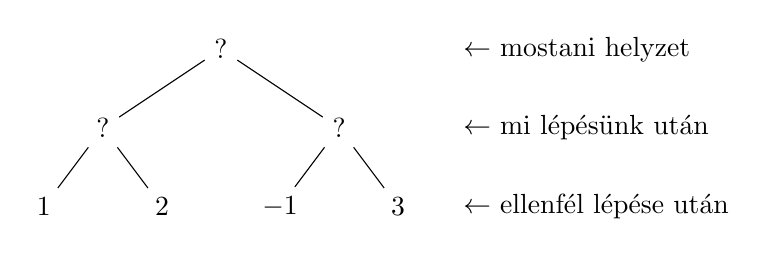
\begin{tikzpicture}[level distance=1cm,
    level 1/.style={sibling distance=3cm},
    level 2/.style={sibling distance=1.5cm}]
  \node (Root) {?}
  child {
    node {?}
    child { node {1} }
    child { node {2} }
  }
  child {
    node {?}
    child { node {$-1$} }
    child { node {3} }
  };
  \begin{scope}[every node/.style={right}]
    \path (Root    -| Root-2-2) node {$\qquad\leftarrow$ mostani helyzet};
    \path (Root-1  -| Root-2-2) node {$\qquad\leftarrow$ mi lépésünk után};
    \path (Root-1-1-| Root-2-2) node {$\qquad\leftarrow$ ellenfél lépése után};
  \end{scope}
\end{tikzpicture}
\end{center}

Itt a mélység 2, tehát 2 lépésre előre gondolkodunk,
és a legmélyebb szinten kiértékelünk minden
állást. Két lépéslehetőségünk van, és ezekre az
ellenfélnek 2-2 válasza. Feltesszük, hogy az
ellenfelünk jól játszik, tehát ha a baloldali lépést
választjuk, arra az ellenfél a saját baloldali (1-es
értékelésű) lépését fogja válaszolni, nem pedig a
jobboldalit, ami nekünk kedvezőbb állást (2)
eredményez. Hasonlóan járunk el a jobboldali
lépésnél: az ellenfél két válasza közül
feltételezzük a kisebbet (-1). Azt láttuk tehát,
hogy a baloldali lépés legrosszabb esetben 1-es, a
jobboldali -1-es értékelésű. Mi nyilván a nagyobbat
választjuk, tehát a mostani helyzetünk 1-es
értékelésű lesz:

\begin{center}
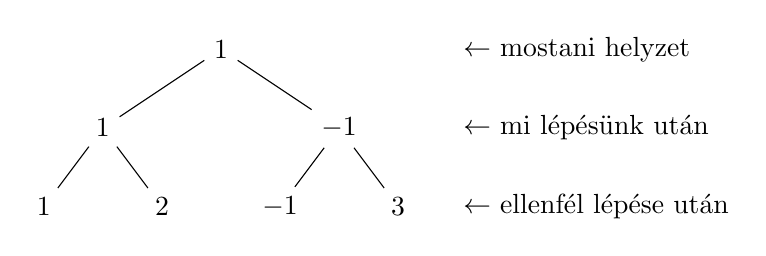
\begin{tikzpicture}[level distance=1cm,
    level 1/.style={sibling distance=3cm},
    level 2/.style={sibling distance=1.5cm}]
  \node (Root) {1}
  child {
    node {1}
    child { node {1} }
    child { node {2} }
  }
  child {
    node {$-1$}
    child { node {$-1$} }
    child { node {3} }
  };
  \begin{scope}[every node/.style={right}]
    \path (Root    -| Root-2-2) node {$\qquad\leftarrow$ mostani helyzet};
    \path (Root-1  -| Root-2-2) node {$\qquad\leftarrow$ mi lépésünk után};
    \path (Root-1-1-| Root-2-2) node {$\qquad\leftarrow$ ellenfél lépése után};
  \end{scope}
\end{tikzpicture}
\end{center}

Ha itt kell lépést választani, akkor a baloldali
mellett döntünk. Ezt a gondolkodást \emph{minimax}
algoritmusnak hívják, mivel az ellenfél lépései
közül a minimális értékűt, a saját lépések közül a
maximális értékűt választjuk.
\index{minimax}

Az alfa--béta nyírás ennek egy hatékonyabb
változata. Itt mindig számon tartjuk azt, hogy mi az
a minimum, amit biztosan el tudunk érni ($\alpha$, a
programban \pr{A}), és mi az a maximum, amit
elérhetünk ($\beta$, a programban \pr{B}), ezek
adják a módszer nevét. Nézzük meg az előbbi példa
kiértékelését, amikor már megvizsgáltuk a teljes
baloldali ágat!

\begin{center}
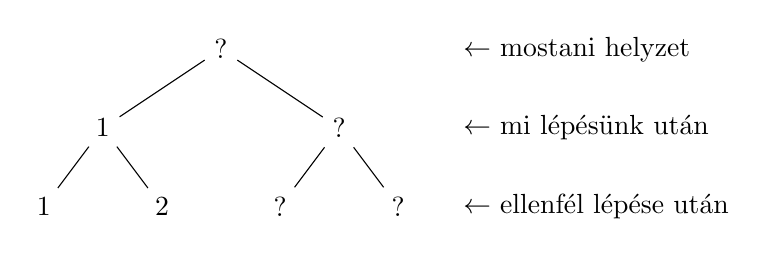
\begin{tikzpicture}[level distance=1cm,
    level 1/.style={sibling distance=3cm},
    level 2/.style={sibling distance=1.5cm}]
  \node (Root) {?}
  child {
    node {1}
    child { node {1} }
    child { node {2} }
  }
  child {
    node {?}
    child { node {?} }
    child { node {?} }
  };
  \begin{scope}[every node/.style={right}]
    \path (Root    -| Root-2-2) node {$\qquad\leftarrow$ mostani helyzet};
    \path (Root-1  -| Root-2-2) node {$\qquad\leftarrow$ mi lépésünk után};
    \path (Root-1-1-| Root-2-2) node {$\qquad\leftarrow$ ellenfél lépése után};
  \end{scope}
\end{tikzpicture}
\end{center}

A jobboldali ággal még egyáltalán nem
foglalkoztunk. Azt tudjuk, hogy ha a baloldali
lépést választjuk, legrosszabb esetben 1-es (tehát
$\alpha=1$). Hogyan módosul ez a jobboldali lépésre
adott baloldali válasz megvizsgálása után?

\begin{center}
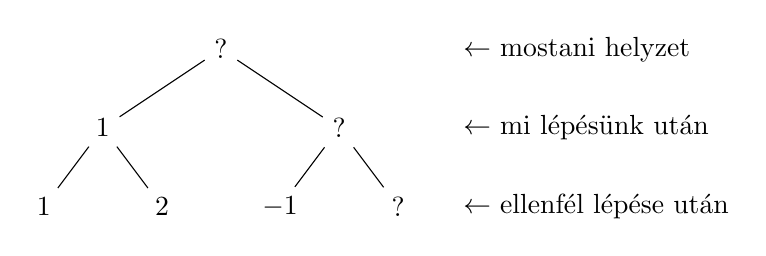
\begin{tikzpicture}[level distance=1cm,
    level 1/.style={sibling distance=3cm},
    level 2/.style={sibling distance=1.5cm}]
  \node (Root) {?}
  child {
    node {1}
    child { node {1} }
    child { node {2} }
  }
  child {
    node {?}
    child { node {$-1$} }
    child { node {?} }
  };
  \begin{scope}[every node/.style={right}]
    \path (Root    -| Root-2-2) node {$\qquad\leftarrow$ mostani helyzet};
    \path (Root-1  -| Root-2-2) node {$\qquad\leftarrow$ mi lépésünk után};
    \path (Root-1-1-| Root-2-2) node {$\qquad\leftarrow$ ellenfél lépése után};
  \end{scope}
\end{tikzpicture}
\end{center}

Azt látjuk, hogy ha a jobboldali lépést választjuk,
akkor legjobb esetben -1-re számíthatunk
($\beta=-1$). Lehet, hogy az ellenfélnek van egy még
erősebb lépése, és a tényleges maximum még kisebb,
de nagyobb nem lehet. Viszont a baloldali ágon már
van egy biztos 1-es, tehát ezt az ágat nem érdemes
tovább vizsgálni, le lehet ,,nyírni''. Általában
tehát ha egy ágon a $\beta$ érték kisebb vagy
egyenlő, mint az eddigi legjobb $\alpha$, akkor nem
kell vele foglalkozni.

Az algoritmust teljesen általánosan meg lehet
fogalmazni, a konkrét játéktól függetlenül. Csak azt
feltételezzük, hogy a következők adottak:
\begin{itemize}
\item \pr{lépés(Állás, Lépés)} : adott állásból
  lehetséges lépés
\item \pr{lép(Lépés, Állás, Állás1)} : adott lépés
  lejátszása
\item \pr{értékelés(Állás, Érték)} : adott állás
  kiértékelése
\end{itemize}

Ebből egyelőre csak a második van meg, a maradék
kettőt a következő részben fogjuk elkészíteni. Most
azonban nézzük az általános algoritmust! Hogy ne
kelljen külön kezelni a minimum- és maximumkereső
eseteket, az értékeléseket minden szintváltáskor
negáljuk. Ahhoz, hogy ez működjön, feltételezzük,
hogy a keresési mélység kezdetben páros, tehát a
0-ás mélységen a pozitív szám jelenti a nekünk jó
állást.

\begin{program}
alfa_béta(0, Állás, _, _, _-Érték) :-
    értékelés(Állás, Érték).
alfa_béta(E, Állás, A, B, Lépés-Érték) :-
    E > 0, E1 is E - 1,
    A1 is -B, B1 is -A,
    findall(L, lépés(Állás, L), Lépések),
    választ(Lépések, Állás, E1, A1, B1,
            nincs, Lépés-Érték).
\end{program}

Ha az előrelátás mélysége 0, akkor az aktuális
állást egyszerűen kiértékeljük. (Ilyenkor a legjobb
lépést jelölő \pr{Lépés} nem kap értéket.) Ha a
mélység legalább 1, akkor eggyel csökkentjük,
negáljuk és megcseréljük az alfát és bétát (hogy a
másik játékos szemszögébe kerüljünk), és választunk
az összes lehetséges lépés közül.

A választást a \pr{választ} végzi:
\begin{program}
választ([], _, _, A, _, Legjobb, Legjobb-A).
választ([Lépés|M], Állás, E, A, B, Legjobb, X) :-
    lép(Lépés, Állás, Állás1),
    alfa_béta(E, Állás1, A, B, _-Érték),
    Érték1 is -Érték,
    nyír(Lépés-Érték1, E, A, B, M, Állás,
         Legjobb, X).
\end{program}

Az utolsóelőtti argumentum az eddigi legjobb lépés
(kezdetben \pr{nincs}), az utolsó pedig a végső
megtalált legjobb lépés és a hozzá tartozó
értékelés.

Ha a lehetséges lépések listája üres, akkor az
eddigi legjobb lépést adja vissza (\pr{Legjobb}) és
a hozzá tartozó érték az \pr{A} lesz. Ha nem
üres, akkor kipróbálja az első lépést: lejátsza, és
az így keletkező állást (rekurzívan) kiértékeli az
\pr{alfa\_béta} szabállyal. Az így kapott
\pr{Érték}-et negálni kell, mert egy szinttel
feljebb léptünk. Végül a \pr{nyír} az eredeti
\pr{Állás} állapotból való lépések közül
(rekurzívan) választ, miközben lenyírja azokat az
ágakat, amelyeket felesleges kiértékelni:
\begin{program}
nyír(Lépés-Érték, _, _, B, _, _, _, Lépés-Érték) :-
    Érték >= B.
nyír(Lépés-Érték, E, A, B, Többi, Állás, _, X) :-
    A < Érték, Érték < B,
    választ(Többi, Állás, E, Érték, B, Lépés, X).
nyír(_-Érték, E, A, B, Többi, Állás, Lépés1, X) :-
    Érték =< A,
    választ(Többi, Állás, E, A, B, Lépés1, X).
\end{program}

Itt három esetet különböztetünk meg, a megvizsgált
lépés értékelésétől függően:
\begin{enumerate}
\item Ha legalább $\beta$, akkor nem kell tovább
  keresni, ennél jobb lépés nem változtat az
  értékelésen. (Ez megfelel annak, hogy a fenti
  példában megtaláltuk a $-1$-et, ami az ellenfél
  számára negálva 1-es, és ezért nem kell még jobb
  lépés után néznie, mert a $\beta$ (a mi negált
  $\alpha$-nk) kisebb, $-1$ értékű.)
\item Ha $\alpha$ és $\beta$ között van, akkor ez
  lesz az eddigi legjobb lépés és az értéke az új
  $\alpha$, és keresünk egy esetleges jobbat a többi
  lépésből.
\item Ha kisebb vagy egyenlő, mint $\alpha$, akkor
  ez a lépés nem érdekes, a többiekben folytatjuk a
  keresést.
\end{enumerate}

\subsection*{Kalah-specifikus részek}
Hogyan tudjuk az összes lehetséges lépést leírni?
\begin{program}
lépés(tábla([0,0,0,0,0,0],_,_,_), []).
lépés(Állás, [L|M]) :-
    tartalmaz(L, [1,2,3,4,5,6]),
    kövek(L, Állás, K),
    lépést_folytat(K, L, Állás, M).
\end{program}
Ha a térfelünk üres, nincs lehetséges lépés. (Erre
azért van szükség, mert a játékot be lehet fejezni
úgy, hogy az utolsó követ a kalahba rakjuk.)
Egyébként a lépés első eleme egy lyukat jelölő 1 és
6 közti szám; a \pr{kövek} biztosítja, hogy van is
benne kő. Azt kell csak ellenőrizni, hogy a kalahba
kerül-e az utolsó, amire a feltétel a 13-al való
osztási maradékkal számolható:
\begin{program}
lépést_folytat(Kövek, L, _, []) :-
    Kövek =\= (7 - L) mod 13, !.
lépést_folytat(Kövek, L, Állás, Lépések) :-
    Kövek =:= (7 - L) mod 13, !,
    vet(Kövek, L, Állás, Állás1),
    lépés(Állás1, Lépések).
\end{program}
Ha a kalahba került, akkor a köveket végigszórjuk,
és ebből az állásból rekurzívan további lépéseket
keresünk.

Egy állás értékelésére egy nagyon egyszerű definíció
a kalahokban levő kövek különbsége:
\begin{program}
értékelés(tábla(_,Na,_,Nb), X) :- X is Na - Nb.
\end{program}

Már csak annyi van hátra, hogy átírjuk a
\pr{lépést\_választ} szabályt. A régi verzió
megmarad arra az esetre, amikor az emberi játékos
van lépésen; a számítógép esetében pedig az
alfa--béta nyírást használjuk:
\begin{program}
lépést_választ(_, ember, Lépés) :-
    nl, kiír('Melyiket választod?'),
    read(Lépés), érvényes(Lépés).
lépést_választ(Állás, számítógép, Lépés) :-
    előrelátás(E),
    alfa_béta(E, Állás, -40, 40, Lépés-_),
    nl, write(Lépés), nl.

előrelátás(4).
\end{program}

Az $[\alpha,\beta]$ intervallumot kezdetben jó
nagyra állítjuk (-40, 40), az előrelátás mélységét
pedig a könnyebb módosíthatóság kedvéért egy külön
tényként tároljuk.

\subsection*{Tesztjáték}
Itt egy 6-os mélységű mesterséges intelligencia
ellen játszott 4-köves játék, ahol a gép kezdett:
\begin{query}
?- kalah.

     4    4    4    4    4    4
0                                  0
     4    4    4    4    4    4

[3,6]

     0    5    5    0    4    4
2                                  0
     5    5    5    5    4    4

Melyiket választod?
|: [2,1].

     0    5    5    0    4    4
2                                  1
     0    1    7    7    6    6

[4]

     1    6    0    0    4    4
3                                  1
     1    2    7    7    6    6

Melyiket választod?
|: [1].

     1    6    0    0    4    4
3                                  1
     0    3    7    7    6    6

[5]

     2    0    0    0    4    4
4                                  1
     1    4    8    8    6    6

Melyiket választod?
|: [2].


     2    0    0    0    4    4
4                                  1
     1    0    9    9    7    7

[6]

     0    0    0    0    4    4
5                                  1
     2    0    9    9    7    7

Melyiket választod?
|: [1].

     0    0    0    0    4    4
5                                  1
     0    1    10   9    7    7

[1]

     0    0    1    1    5    0
7                                  1
     0    0    10   9    7    7

Melyiket választod?
|: [5].

     0    1    2    2    6    1
7                                  2
     0    0    10   9    0    8

[1]

     0    1    2    2    7    0
7                                  2
     0    0    10   9    0    8

Melyiket választod?
|: [6].

     0    2    3    3    8    1
7                                  5
     0    0    10   9    0    0

[5,6,4,6,1]

     0    1    0    3    9    0
11                                 5
     0    0    10   9    0    0

Melyiket választod?
|: [3].

     1    2    1    4    10   1
11                                 6
     0    0    0    10   1    1

[6,5,4]

     1    1    0    4    10   1
13                                 6
     0    0    0    10   1    1

Melyiket választod?
|: [4].

     0    2    1    5    11   2
13                                 10
     0    0    0    0    2    2

[1]

     0    2    1    6    12   0
13                                 10
     0    0    0    0    2    2

Melyiket választod?
|: [6].

     0    2    1    6    12   1
13                                 11
     0    0    0    0    2    0

[1]

     0    2    1    6    13   0
13                                 11
     0    0    0    0    2    0

Melyiket választod?
|: [5,6].

     0    0    0    0    0    0
35                                 13
     0    0    0    0    0    0
Nyertem.
\end{query}

\begin{problem}
Írd át a játékos lépését, hogy hibás lépés
esetén kérdezzen újra, és \pr{kilépés}-re lépjen ki!
\end{problem}
\begin{problem}
Készíts szigorúbb ellenőrzést az emberi játékos
lépéseihez, ami (i) nem enged üres lyukat
választani, és (ii) akkor és csak akkor enged több
lépést, ha az utolsó kő a kalahba kerül!
\end{problem}
\begin{problem}
Írd át a programot úgy, hogy a bonyolultabb (de
izgalmasabb) Oware játék szabályait kövesse!  A
különbségek:
\begin{itemize}
\item A kövek száma általában lyukanként 4
\item A szórásnál a kalahokat és a kezdő lyukat ki kell hagyni
\item Követ úgy lehet szerezni, hogy ha olyan helyre
  érkezünk, ami (i) az ellenfél oldalán van és (ii)
  a szórás befejeztével 2 vagy 3 kő lesz benne.  Ha
  ez teljesül, akkor az ebben levő összes követ
  megkapjuk, sőt, ha az előzőre is teljesül, akkor
  az abban levőket is és így tovább, amíg igaz a két
  feltétel.
\item Ha lehet, muszáj olyat lépnünk, hogy az
  ellenfél oldalán maradjon kő. Ha nem lehet, akkor
  a maradék köveket megkapjuk.
\end{itemize}
\end{problem}
\begin{problem}
Írj dámajátékot! A játék kerete legyen ugyanaz,
és a számítógép használja a fenti alfa--béta nyírás
algoritmust.
\end{problem}

\subsection*{A teljes program}
\begin{program}
% Magas szintű keretprogram

kalah :-
    alapbeállítás(Állás, Játékos),
    kirajzol(Állás, Játékos),
    játék(Állás, Játékos).

játék(Állás, Játékos) :-
    játék_vége(Állás, Játékos, Eredmény), !,
    bejelent(Eredmény).
játék(Állás, Játékos) :-
    lépést_választ(Állás, Játékos, Lépés),
    lép(Lépés, Állás, Állás1),
    következő_játékos(Játékos, Játékos1), !,
    kirajzol(Állás1, Játékos1),
    játék(Állás1, Játékos1).

következő_játékos(ember, számítógép).
következő_játékos(számítógép, ember).

bejelent(ember) :- kiír('Nyertél, gratulálok!').
bejelent(számítógép) :- kiír('Nyertem.').
bejelent(döntetlen) :- kiír('Döntetlen lett!').

% Reprezentáció

alapbeállítás(Állás, ember) :-
    kövek_száma(K),
    Állás = tábla([K,K,K,K,K,K],0,
                  [K,K,K,K,K,K],0).

% Szabályok

játék_vége(tábla(_,N,_,N), _, döntetlen) :-
    kövek_száma(K), N =:= 6 * K, !.
játék_vége(tábla(_,N1,_,_), Játékos, Játékos) :-
    kövek_száma(K), N1 > 6 * K, !.
játék_vége(tábla(_,_,_,N2), Játékos, Másik) :-
    kövek_száma(K), N2 > 6 * K,
    következő_játékos(Játékos, Másik).

lép([], Állás, Állás1) :- megfordít(Állás, Állás1).
lép([L|M], Állás, Állás2) :-
    kövek(L, Állás, K),
    vet(K, L, Állás, Állás1),
    lép(M, Állás1, Állás2).

megfordít(tábla(La,Na,Lb,Nb), tábla(Lb,Nb,La,Na)).

kövek(I, tábla(L,_,_,_), K) :- n_edik(I, L, K), K > 0.

vet(Kövek, Luk, Állás, Állás2) :-
    vet_saját(Kövek, Luk, Állás, Állás1, Kövek1),
    vet_ellenfél(Kövek1, Állás1, Állás2).

vet_saját(Kövek, Luk, tábla(La,Na,Lb,Nb),
          tábla(La1,Na1,Lb,Nb), Kövek1) :-
    Kövek > 7 - Luk, !, % átmegy az ellenfélhez
    felvesz_és_szór(Luk, Kövek, La, La1),
    Na1 is Na + 1, Kövek1 is Kövek + Luk - 7.
vet_saját(Kövek, Luk,
          tábla(La,Na,Lb,Nb), Állás, 0) :-
    Kövek =< 7 - Luk,
    felvesz_és_szór(Luk, Kövek, La, La1),
    elfogás(Luk, Kövek, La1, La2, Lb, Lb1, N),
    raktározás(N, Kövek, Luk, Na, Na1),
    vetés_vége(tábla(La2,Na1,Lb1,Nb), Állás).

felvesz_és_szór(0, K, L, L1) :- % szórás folytatása
    !, szór(K, L, L1).
felvesz_és_szór(1, K, [_|M], [0|M1]) :-
    !, szór(K, M, M1).
felvesz_és_szór(Luk, K, [L|M], [L|M1]) :-
    Luk > 1, !, Luk1 is Luk - 1,
    felvesz_és_szór(Luk1, K, M, M1).

szór(0, L, L) :- !.
szór(N, [L|M], [L1|M1]) :-
    N > 0, !,
    N1 is N - 1, L1 is L + 1,
    szór(N1, M, M1).
szór(_, [], []) :- !.

elfogás(Luk, Kövek, La, La1, Lb, Lb1, N) :-
    Vége is Luk + Kövek,
    n_edik(Vége, La, 1),
    Szemben is 7 - Vége,
    n_edik(Szemben, Lb, K),
    K > 0, !, % üresbe érkeztünk és van szemben kő
    n_csere(Vége, La, 0, La1),
    n_csere(Szemben, Lb, 0, Lb1),
    N is K + 1.
elfogás(_, _, La, La, Lb, Lb, 0) :- !.

raktározás(0, Kövek, Luk, Na, Na) :-
    Kövek < 7 - Luk, !.
raktározás(0, Kövek, Luk, Na, Na1) :-
    Kövek =:= 7 - Luk, !, Na1 is Na + 1.
raktározás(N, _, _, Na, Na1) :-
    N > 0, !, Na1 is Na + N.

vetés_vége(tábla(La,Na,Lb,Nb),
           tábla(La,Na,La,Nb1)) :-
    üres(La), !, összeg(Lb, X), Nb1 is Nb + X.
vetés_vége(tábla(La,Na,Lb,Nb),
           tábla(Lb,Na1,Lb,Nb)) :-
    üres(Lb), !, összeg(La, X), Na1 is Na + X.
vetés_vége(Állás, Állás) :- !.

üres([0,0,0,0,0,0]).

vet_ellenfél(0, Állás, Állás) :- !.
vet_ellenfél(Kövek, tábla(La,Na,Lb,Nb),
             tábla(La,Na,Lb1,Nb)) :-
    1 =< Kövek, Kövek =< 6,
    \+ üres(La), !,
    szór(Kövek, Lb, Lb1).
vet_ellenfél(Kövek, tábla(La,Na,Lb,Nb),
             tábla(La,Na,La,Nb1)) :-
    1 =< Kövek, Kövek =< 6,
    üres(La), !,
    összeg(Lb, X), Nb1 is Nb + Kövek + X.
vet_ellenfél(Kövek, tábla(La,Na,Lb,Nb), Állás) :-
    Kövek > 6, !,
    szór(6, Lb, Lb1),
    Kövek1 is Kövek - 6,
    vet(Kövek1, 0, tábla(La,Na,Lb1,Nb), Állás).

% Kirajzolás

kirajzol(Állás, számítógép) :- kirajzol(Állás).
kirajzol(Állás, ember) :-
    megfordít(Állás, Állás1),
    kirajzol(Állás1).

kirajzol(tábla(La,Na,Lb,Nb)) :-
    nl,
    fordított(La, F),
    sort_ír(F),
    kalahot_ír(Na, Nb),
    sort_ír(Lb).

sort_ír(L) :- behúz(5), lyukat_ír(L).

lyukat_ír([]) :- nl.
lyukat_ír([L|M]) :- köveket_ír(L), lyukat_ír(M).

köveket_ír(N) :- N < 10, write(N), behúz(4).
köveket_ír(N) :- N >= 10, write(N), behúz(3).

kalahot_ír(N1, N2) :-
    köveket_ír(N1), behúz(30),
    write(N2), nl.

% Alfa-béta nyírás

alfa_béta(0, Állás, _, _, _-Érték) :-
    értékelés(Állás, Érték).
alfa_béta(E, Állás, A, B, Lépés-Érték) :-
    E > 0, E1 is E - 1,
    A1 is -B, B1 is -A,
    findall(L, lépés(Állás, L), Lépések),
    választ(Lépések, Állás, E1, A1, B1,
            nincs, Lépés-Érték).

választ([], _, _, A, _, Legjobb, Legjobb-A).
választ([Lépés|M], Állás, E, A, B, Legjobb, X) :-
    lép(Lépés, Állás, Állás1),
    alfa_béta(E, Állás1, A, B, _-Érték),
    Érték1 is -Érték,
    nyír(Lépés-Érték1, E, A, B, M, Állás,
         Legjobb, X).

nyír(Lépés-Érték, _, _, B, _, _, _, Lépés-Érték) :-
    Érték >= B.
nyír(Lépés-Érték, E, A, B, Többi, Állás, _, X) :-
    A < Érték, Érték < B,
    választ(Többi, Állás, E, Érték, B, Lépés, X).
nyír(_-Érték, E, A, B, Többi, Állás, Lépés1, X) :-
    Érték =< A,
    választ(Többi, Állás, E, A, B, Lépés1, X).

% Kalah-specifikus rész

lépés(tábla([0,0,0,0,0,0],_,_,_), []).
lépés(Állás, [L|M]) :-
    tartalmaz(L, [1,2,3,4,5,6]),
    kövek(L, Állás, K),
    lépést_folytat(K, L, Állás, M).

lépést_folytat(Kövek, L, _, []) :-
    Kövek =\= (7 - L) mod 13, !.
lépést_folytat(Kövek, L, Állás, Lépések) :-
    Kövek =:= (7 - L) mod 13, !,
    vet(Kövek, L, Állás, Állás1),
    lépés(Állás1, Lépések).

értékelés(tábla(_,Na,_,Nb), X) :- X is Na - Nb.

lépést_választ(_, ember, Lépés) :-
    nl, kiír('Melyiket választod?'),
    read(Lépés), érvényes(Lépés).
lépést_választ(Állás, számítógép, Lépés) :-
    előrelátás(E),
    alfa_béta(E, Állás, -40, 40, Lépés-_),
    nl, write(Lépés), nl.

érvényes([]).
érvényes([L|M]) :- 0 < L, L < 7, érvényes(M).

% Beállítások

kövek_száma(6).

előrelátás(4).

% Segéd-szabályok

kiír(X) :- write(X), nl.

behúz(0) :- !.
behúz(N) :-
    N > 0, N1 is N - 1,
    write(' '), behúz(N1).

tartalmaz(X, [X|_]).
tartalmaz(X, [_|Maradék]) :- tartalmaz(X, Maradék).

fordított(X, Y) :- fordított(X, [], Y).

fordított([], Y, Y).
fordított([X|M], F, Y) :- fordított(M, [X|F], Y). 

n_edik(N, [_|M], X) :-
    N > 1, !, N1 is N - 1,
    n_edik(N1, M, X).
n_edik(1, [X|_], X).

n_csere(1, [_|M], Y, [Y|M]) :- !.
n_csere(N, [X|M], Y, [X|M1]) :-
    N > 1, !, N1 is N - 1,
    n_csere(N1, M, Y, M1).

összeg(L, X) :- összeg(L, 0, X).

összeg([], A, A).
összeg([K|M], A, X) :-
    A1 is A + K,
    összeg(M, A1, X).
\end{program}
